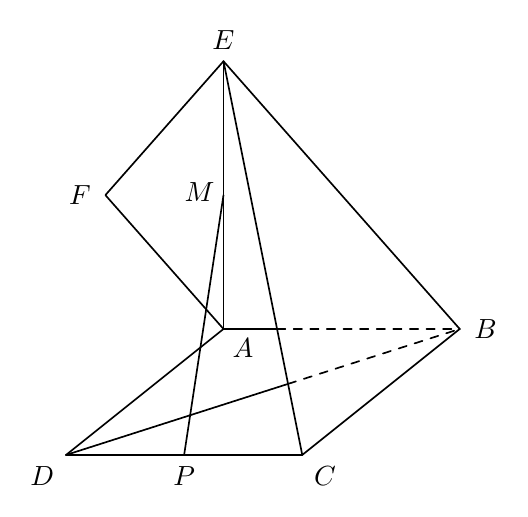
\begin{tikzpicture}[line width=.6pt, line join=round, line cap=round]
% 正方形 ABCD 与四边形 ABEF, E 顶点, M 在 EA 上, P 在 DC 上
\coordinate (E) at (3.0,5.2);
\coordinate (A) at (3.0,1.8);
\coordinate (B) at (6.0,1.8);
\coordinate (D) at (1.0,0.2);
\coordinate (C) at (4,0.2);
\coordinate (F) at (1.5,3.5);
\coordinate (M) at (3,3.5);
\coordinate (P) at (2.5,0.2);
\coordinate (ABmid) at (3.68,1.8);
% upper part
\draw (E) -- (F) -- (A);
\draw (E) -- (A);
\draw (E) -- (B);
\draw (E) -- (C);
% square ABCD: A-B solid then dashed near B, B-C, C-D, D-A
\draw (A) -- (ABmid);
\draw[dashed] (ABmid) -- (B);
\draw (B) -- (C);
\draw (D) -- (C);
\draw (A) -- (D);
% diagonal D-B (solid left, dashed near B)
\draw (D) -- (3.819548872,1.102255639);
\draw[dashed] (3.819548872,1.102255639) -- (B);
% M-P
\draw (M) -- (P);
% labels with clearance
\node[font=\normalsize, inner sep=1pt, above, yshift=3pt] at (E) {$E$};
\node[font=\normalsize, inner sep=1pt, left, xshift=-4pt] at (F) {$F$};
\node[font=\normalsize, inner sep=1pt, left, xshift=-2pt, yshift=1pt] at (M) {$M$};
\node[font=\normalsize, inner sep=1pt, below right=2pt] at (A) {$A$};
\node[font=\normalsize, inner sep=1pt, right, xshift=4pt] at (B) {$B$};
\node[font=\normalsize, inner sep=1pt, below left, xshift=-3pt, yshift=-3pt] at (D) {$D$};
\node[font=\normalsize, inner sep=1pt, below right, xshift=3pt, yshift=-3pt] at (C) {$C$};
\node[font=\normalsize, inner sep=1pt, below, yshift=-3pt] at (P) {$P$};
\end{tikzpicture}
